\chapter{ Технологический раздел}
\label{cha:technological}

    В данном разделе будут выбраны средства реплизации ПО, представлен листинг кода
    и проведён теоритический анализ максимальной затрачиваемой памяти. 

    \section{Средства реализации}
        В данной работе используется язык программирования C++, так как
        язык позволяет написать программу, работающую относительно быстро. 
        Проект выполнен в IDE CLion \cite{visual-studio}.

        Для замера процессорного времени была использована функция getCPUTime \cite{getCPUTime}
        реализованная David Robert Nadeau для Linux и Windows , использование которой представлено в листинге \ref{lst:getCPUTime}.

        \begin{lstlisting}[language=C++, label=lst:getCPUTime, caption=Функция замера времени]

/*
* Author:  David Robert Nadeau
* Site:    http://NadeauSoftware.com/
* License: Creative Commons Attribution 3.0 Unported License
*          http://creativecommons.org/licenses/by/3.0/deed.en_US
*/
#if defined(_WIN32)
#include <Windows.h>

#elif defined(__unix__) || defined(__unix) || defined(unix) || (defined(__APPLE__) && defined(__MACH__))
#include <unistd.h>
#include <sys/resource.h>
#include <sys/times.h>
#include <time.h>

#else
#error "Unable to define getCPUTime( ) for an unknown OS."
#endif

/**
* Returns the amount of CPU time used by the current process,
* in seconds, or -1.0 if an error occurred.
*/
double getCPUTime( )
{
#if defined(_WIN32)
/* Windows -------------------------------------------------- */
FILETIME createTime;
FILETIME exitTime;
FILETIME kernelTime;
FILETIME userTime;
if ( GetProcessTimes( GetCurrentProcess( ),
&createTime, &exitTime, &kernelTime, &userTime ) != -1 )
{
SYSTEMTIME userSystemTime;
if ( FileTimeToSystemTime( &userTime, &userSystemTime ) != -1 )
return (double)userSystemTime.wHour * 3600.0 +
(double)userSystemTime.wMinute * 60.0 +
(double)userSystemTime.wSecond +
(double)userSystemTime.wMilliseconds / 1000.0;
}

#elif defined(__unix__) || defined(__unix) || defined(unix) || (defined(__APPLE__) && defined(__MACH__))
/* AIX, BSD, Cygwin, HP-UX, Linux, OSX, and Solaris --------- */

#if defined(_POSIX_TIMERS) && (_POSIX_TIMERS > 0)
/* Prefer high-res POSIX timers, when available. */
{
clockid_t id;
struct timespec ts;
#if _POSIX_CPUTIME > 0
/* Clock ids vary by OS.  Query the id, if possible. */
if ( clock_getcpuclockid( 0, &id ) == -1 )
#endif
#if defined(CLOCK_PROCESS_CPUTIME_ID)
/* Use known clock id for AIX, Linux, or Solaris. */
id = CLOCK_PROCESS_CPUTIME_ID;
#elif defined(CLOCK_VIRTUAL)
/* Use known clock id for BSD or HP-UX. */
id = CLOCK_VIRTUAL;
#else
id = (clockid_t)-1;
#endif
if ( id != (clockid_t)-1 && clock_gettime( id, &ts ) != -1 )
return (double)ts.tv_sec +
(double)ts.tv_nsec / 1000000000.0;
}
#endif

#if defined(RUSAGE_SELF)
{
struct rusage rusage;
if ( getrusage( RUSAGE_SELF, &rusage ) != -1 )
return (double)rusage.ru_utime.tv_sec +
(double)rusage.ru_utime.tv_usec / 1000000.0;
}
#endif

#if defined(_SC_CLK_TCK)
{
const double ticks = (double)sysconf( _SC_CLK_TCK );
struct tms tms;
if ( times( &tms ) != (clock_t)-1 )
return (double)tms.tms_utime / ticks;
}
#endif

#if defined(CLOCKS_PER_SEC)
{
clock_t cl = clock( );
if ( cl != (clock_t)-1 )
return (double)cl / (double)CLOCKS_PER_SEC;
}
#endif

#endif

return -1;      /* Failed. */
}        \end{lstlisting}

    \section{Листинг программы}
        Ниже представлены листинги кода поиска растояния Левенштейна: \begin{enumerate}
            \item нерекурсивного с заполнением матрицы (листинг \ref{lst:matr:Levenstein});
            \item рекурсивного без заполнения матрицы (листинг \ref{lst:rec:Levenstein});
            \item рекурсивного с заполнением матрицы (листинг \ref{lst:rec-matr:Levenstein});
        \end{enumerate}
        
        и код функции поиска растояния Дамерау-Левенштейна (листинг \ref{lst:matr:Dameray-Levenstein}).

        \begin{lstlisting}[language=C++, label=lst:matr:Levenstein, caption=Функция нерекурсивного поиска с заполнением матрицы]
size_t Levenshtein::withoutRecursion(const std::string& str1, const std::string& str2, bool debugMode) {
    auto len1 = str1.length();
    auto len2 = str2.length();
    auto matrix = Matrix(len1 + 1, len2 + 1);

    for (size_t i = 0; i <= len1; i++)
        matrix[i][0] = i;
    for (size_t j = 0; j <= len2; j++)
        matrix[0][j] = j;

    for (auto i = 1; i <= len1; i++)
    {
        for (auto j = 1; j <= len2; j++)
        {
            auto m = 1;
            if (str1[i - 1] == str2[j - 1])
                m = 0;

            matrix[i][j] = std::min(matrix[i - 1][j] + 1,
            std::min(matrix[i][j - 1] + 1,
            matrix[i - 1][j - 1] + m));
        }
    }
    if (debugMode) {
        std::cout << "Levenshtein without recursion" << std::endl;
        matrix.print();
    }
    return matrix[len1][len2];
}
        \end{lstlisting}

        \begin{lstlisting}[language=C++, label=lst:rec:Levenstein, caption=Функция рекурсивного поиска без заполнения матрицы]
size_t Levenshtein::_recursionWithoutCash(const char* str1, size_t i, const char* str2, size_t j) {
    size_t res;
    if (i)
    {
        if (j)
        {
            auto m = 1;
            if (str1[i - 1] == str2[j - 1])
            m = 0;

            auto a = _recursionWithoutCash(str1, i, str2, j - 1) + 1;
            auto b = _recursionWithoutCash(str1, i - 1, str2, j) + 1;
            auto c = _recursionWithoutCash(str1, i - 1, str2, j - 1) + m;
            res = std::min(a, std::min(b, c));
        }
        else
            res = i;
    }
    else
        res = j;
    return res;
}

size_t Levenshtein::recursionWithoutCash(const std::string &str1, const std::string &str2) {
    auto i = str1.length();
    auto j = str2.length();
    return _recursionWithoutCash(str1.data(), i, str2.data(), j);
}
        \end{lstlisting}

        \begin{lstlisting}[language=C++, label=lst:rec-matr:Levenstein, caption=Функция рекурсивного поиска с заполнением матрицы]

size_t Levenshtein::recursionWithCash(const std::string &str1, const std::string &str2, bool debugMode) {
    auto n = str1.length();
    auto m = str2.length();

    auto matrix = Matrix(n + 1, m + 1);
    for (size_t i = 0; i <= n; i++)
    {
        for (size_t j = 0; j <= m; j++)
            matrix[i][j] = -1;
    }

    auto res = _recursionWithCash(str1.data(), n, str2.data(), m, matrix);
    if (debugMode) {
        std::cout << "Levenshtein recursion with cash" << std::endl;
        matrix.print();
    }
    return res;
}

size_t Levenshtein::_recursionWithCash(const char* str1, size_t i, const char* str2, size_t j, Matrix& matrix) {

    if (!i)
        matrix[i][j] = j;
    else if (!j)
        matrix[i][j] = i;
    else
    {
        if (matrix[i][j - 1] == -1)
            matrix[i][j - 1] = _recursionWithCash(str1, i, str2, j - 1, matrix);
        if (matrix[i - 1][j] == -1)
            matrix[i - 1][j] = _recursionWithCash(str1, i - 1, str2, j, matrix);
        if (matrix[i - 1][j - 1] == -1)
            matrix[i - 1][j - 1] = _recursionWithCash(str1, i - 1, str2, j - 1, matrix);
        matrix[i][j] = std::min(std::min(matrix[i][j - 1], matrix[i - 1][j]) + 1,
                                matrix[i - 1][j - 1] + (str1[i - 1] != str2[j - 1]));
    }

    return matrix[i][j];
}
        \end{lstlisting}

        \begin{lstlisting}[language=C++, label=lst:matr:Dameray-Levenstein, caption=Функция поиска растояния Дамерау-Левенштейна]

size_t Levenshtein::recursionDamerauWithoutCash(const std::string &str1, const std::string &str2) {
    auto i = str1.length();
    auto j = str2.length();

    return _recursionDamerauWithoutCash(str1.data(), i, str2.data(), j);
}

size_t Levenshtein::_recursionDamerauWithoutCash(const char* str1, size_t i, const char* str2, size_t j) {
    size_t res;
    if (i)
    {
        if (j)
        {
            auto m = 1;
            if (str1[i - 1] == str2[j - 1])
                m = 0;

            auto a = _recursionWithoutCash(str1, i, str2, j - 1) + 1;
            auto b = _recursionWithoutCash(str1, i - 1, str2, j) + 1;
            auto c = _recursionWithoutCash(str1, i - 1, str2, j - 1) + m;
            res = std::min(a, std::min(b, c));
            if (i > 1 && j > 1 && str1[i - 1] == str2[j - 2] && str1[i - 2] == str2[j - 1])
                res = std::min(res, _recursionWithoutCash(str1, i - 2, str2, j - 2) + 1);
        }
        else
            res = i;
    }
    else
        res = j;
    return res;
}
        \end{lstlisting}
    
        
    \section{Тестирование}
        В таблице \ref{table:testing} отображён возможный набор тестов
        для тестирования методом чёрного ящика, результаты которого, 
        представленные на рисунке \ref{png:testing:result}, подтверждают
        прохождение программы перечисленных тестов.
        \begin{table}[]
            \caption{Тесты проверки корректности программы}
            \centering
            \begin{tabular}{|c|c|c|c|c|}
            \hline
            № & строка 1 & строка 2 & \begin{tabular}[c]{@{}c@{}}Ожидаемый результат \\ (р.Л, р.Д-Л)\end{tabular} & \begin{tabular}[c]{@{}c@{}}Фактический результат\\ (р.Л, р.Д-Л)\end{tabular} \\ \hline
            1 & 0        & 0        & 0, 0                                                                        & 0, 0                                                                         \\ \hline
            2 & 0        & ab       & 2, 2                                                                        & 2, 2                                                                         \\ \hline
            3 & abba     & baab     & 3, 2                                                                        & 3, 2                                                                         \\ \hline
            4 & abcd     & qwer     & 4, 4                                                                        & 4, 4                                                                         \\ \hline
            \end{tabular}
            \label{table:testing}
        \end{table}

        \begin{figure}[h!]
            \centering
            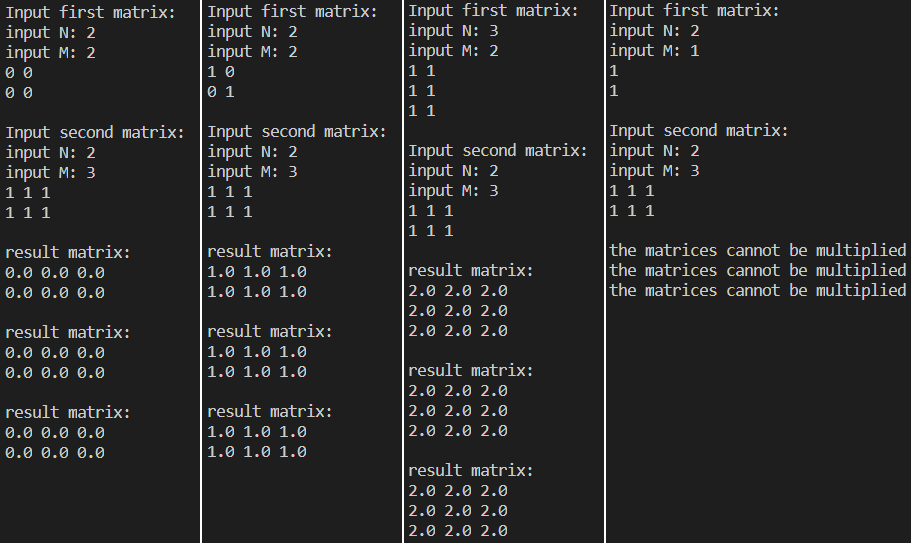
\includegraphics[scale=1.2]{testing.png}
            \caption{Результаты тестирования}
            \label{png:testing:result}
        \end{figure}

    \section{Сравнительный анализ потребляемой памяти}  
        С точки зрения использования памяти алгоритмы Левенштейна и
        Дамерау-Левенштейна не отличаются, следовательно, достаточно
        рассмотреть лишь разницу рекурсивной и матричной реализаций
        данных методов.
        
        Использование памяти на строках $s_1$, $s_2$ длиной n и m соответственно
        при использовании матрицы теоритически определяется формулой (\ref{formula:memory:matr}):
        \begin{equation}
            V = (n + 1)(m + 1)sizeof(int) + 4sizeof(size\_t) + 2sizeof(char*) + sizeof(char)(n + m)
            \label{formula:memory:matr}
        \end{equation}
        

        Максимальный расход памяти памяти на строках $s_1$, $s_2$ длиной n и m соответственно
        при использовании рекурсии определяется максимальной глибиной стека вызовов,
        которая теоритически определяется формулой (\ref{formula:memory:rec}):
        \begin{equation}
            V = sizeof(char)(n + m)  + (n + m)(2sizeof(char*) + 3sizeof(size\_t))
            \label{formula:memory:rec}
        \end{equation}
\newpage